\documentclass[11pt]{article}

\usepackage[margin=1in]{geometry}
\usepackage{graphicx}
\usepackage{booktabs}
\usepackage{array}
\usepackage{hyperref}
\usepackage{xcolor}
\usepackage{float}

\hypersetup{hidelinks,hypertexnames=false}
\graphicspath{{../artifacts/showcase/}}

\title{LoopPlane: Durable Objective-Gated Agent Workflows}
\author{LoopPlane Project}
\date{June 16, 2026}

\begin{document}
\maketitle

\begin{abstract}
LoopPlane is a local runtime for durable agent loop engineering. It packages
agent work as a portable workflow product: a static execution plan, semantic
objective gates, agent-produced evidence, bounded self-expansion, read-model
projections, and user-friendly review surfaces. The core architecture separates
local workflow truth from semantic agent judgment and from presentation
surfaces, so workflows can be moved, resumed, reviewed, and handed off with
their reasoning trail intact.
\end{abstract}

\section{Product Thesis}

LoopPlane is designed for projects where a one-shot agent prompt is not enough.
The workflow needs to keep working, preserve evidence, verify high-level
delivery, expand when the result is incomplete, and remain usable by people who
did not watch the run happen.

\begin{figure}[H]
\centering
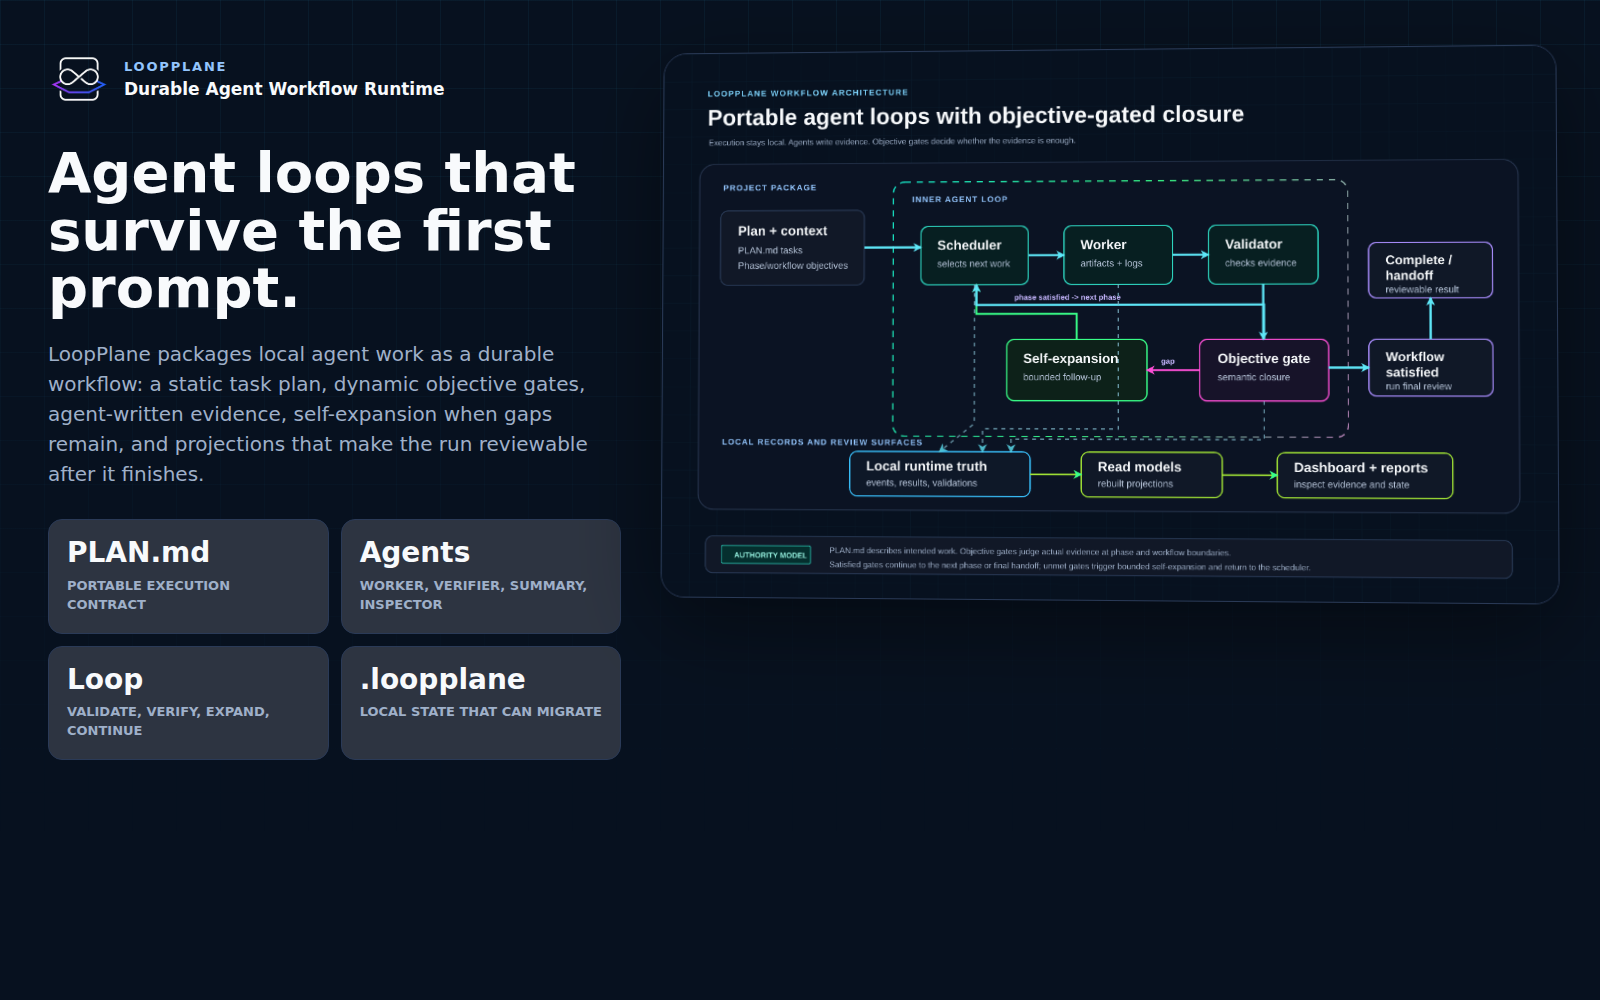
\includegraphics[width=\linewidth]{showcase_hero.png}
\caption{LoopPlane packages agent work as a durable loop: portable plan,
objective gates, local evidence, bounded expansion, and reviewable
projections.}
\end{figure}

The product promise is straightforward:

\begin{itemize}
\item the plan and runtime records live with the project;
\item machine-specific runner paths and secrets stay local;
\item objective closure is judged from actual evidence;
\item incomplete objectives can produce scoped follow-up work;
\item dashboards, summaries, graphs, and reports make the loop usable without
becoming the source of truth.
\end{itemize}

\section{Workflow Architecture}

Figure~\ref{fig:architecture} shows the workflow architecture. Execution writes
local truth. Objective gates judge that truth. Self-expansion extends the plan
when a gap remains. Read models and operator surfaces are rebuilt from local
records.

\begin{figure}[H]
\centering
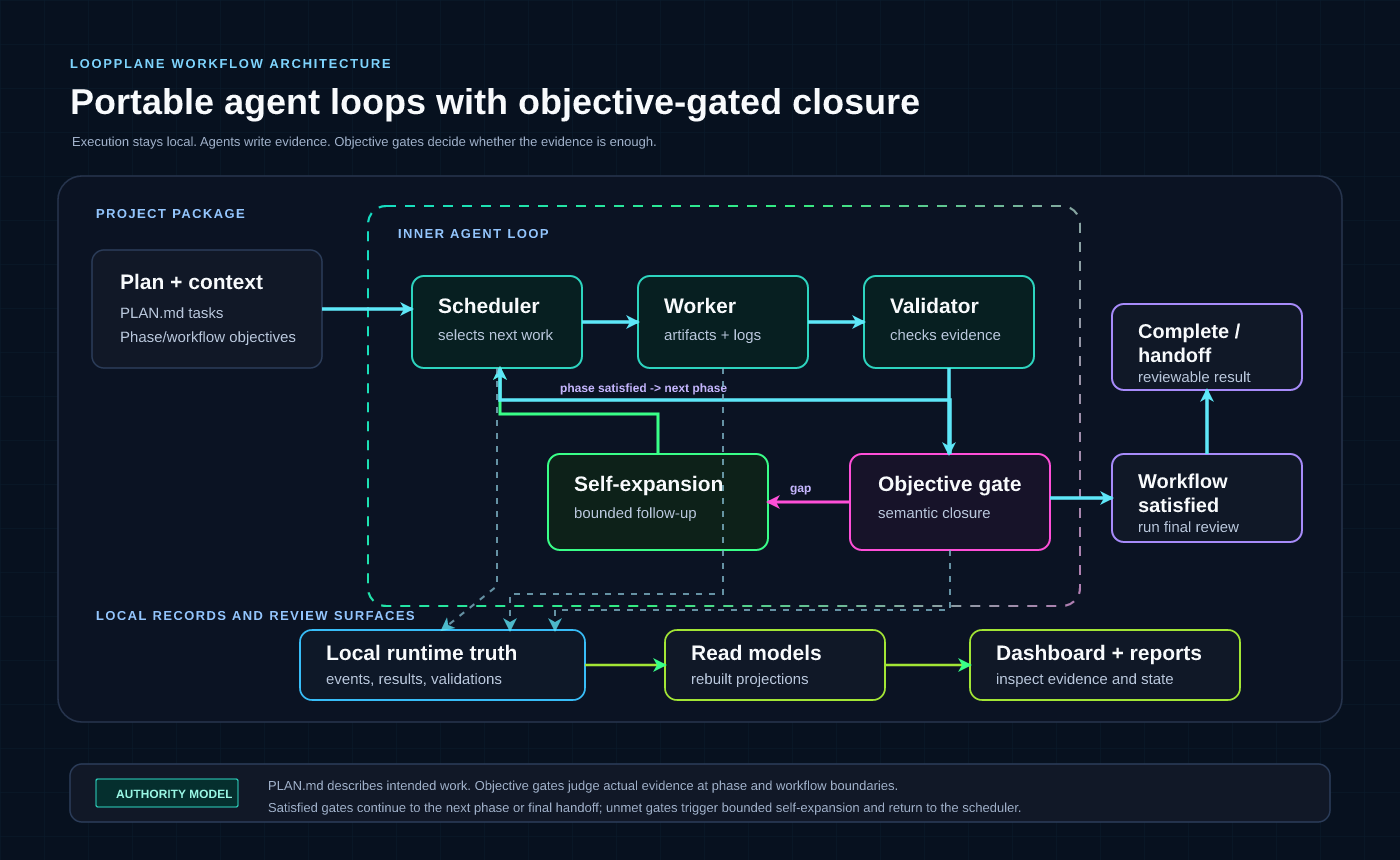
\includegraphics[width=\linewidth]{loopplane_workflow_diagram.png}
\caption{LoopPlane architecture. Local runtime records are authoritative;
objective gates and summaries are semantic agent judgments; read models power
review surfaces such as dashboards, summaries, graphs, and reports.}
\label{fig:architecture}
\end{figure}

\subsection{Authority Boundaries}

\begin{table}[H]
\centering
\begin{tabular}{p{0.24\linewidth}p{0.32\linewidth}p{0.34\linewidth}}
\toprule
Layer & Examples & Product Role \\
\midrule
Execution contract & \texttt{PLAN.md}, brief, shared context & Describes tasks, phases, objectives, dependencies, and intent. \\
Runtime truth & Events, leases, state, results, validations, objective reports, expansion registry & Records what happened and what was accepted. \\
Semantic agents & Worker, validator, objective verifier, summary, inspector, expansion planner & Interpret evidence and propose or judge outcomes. \\
Review surfaces & Dashboard, graph, metrics, summaries, technical reports & Help users understand and operate the workflow. \\
\bottomrule
\end{tabular}
\caption{LoopPlane separates workflow authority from review surfaces.}
\end{table}

\section{Static Plan, Dynamic Delivery}

LoopPlane combines a static execution contract with dynamic delivery judgment.
\texttt{PLAN.md} is stable enough for the scheduler to run deterministically:
tasks have dependencies, evidence locations, deliverables, risk, and validation
strategy. Objectives are higher-level delivery expectations checked after a
phase or full workflow boundary.

This distinction is central. A worker can complete a task mechanically while
still leaving a semantic delivery gap. LoopPlane therefore uses objective
verifier agents to judge whether the actual evidence satisfies the objective,
rather than treating checklist completion as sufficient.

\section{Runtime Loop}

The scheduler keeps the workflow durable:

\begin{enumerate}
\item load the active workflow state and active plan;
\item select a runnable task, objective gate, expansion action, recovery step,
or control request;
\item prepare a run directory and active lease;
\item invoke the configured agent runner through an adapter;
\item classify output and status files;
\item append events and update runtime state;
\item run validation or objective verification when a boundary is reached;
\item rebuild read models from local workflow records.
\end{enumerate}

The scheduler is intentionally mechanical. It preserves ordering, leases,
events, schemas, and replayable state. Semantic interpretation remains with
agents.

\section{Objective-Gated Self-Expansion}

Objective-gated self-expansion is the mechanism that turns an incomplete result
into bounded follow-up work.

\begin{itemize}
\item The objective verifier reads the selected objectives, plan context, task
records, artifact inventory, prior objective reports, and expansion history.
\item It records whether each objective is satisfied, waived, partial, blocked,
or expandable.
\item Expandable gaps can trigger the expansion planner.
\item The expansion planner emits a proposal and a bounded plan patch.
\item Policy controls whether the patch can be applied automatically or must be
approved.
\item Applied patches return to the scheduler as executable work.
\end{itemize}

This keeps the loop moving without hiding the reason it moved. Expansion is a
recorded workflow event, not an invisible retry.

\section{Agent Runner Inheritance}

LoopPlane treats semantic roles as first-class agent roles. Planner, worker,
validator, objective verifier, summary, final reviewer, inspector, and
expansion planner roles inherit the configured default runner unless a project
explicitly overrides them. A user who configures a Codex or Claude CLI runner
should not have to configure every role by hand before the workflow becomes
usable.

\section{Review Surfaces}

LoopPlane includes a dashboard because durable agent work must be easy to
review. The dashboard is an operator surface over local records: it shows
objective closure, task evidence, graph history, summaries, runner state,
approvals, and change requests in one place.

\begin{figure}[H]
\centering
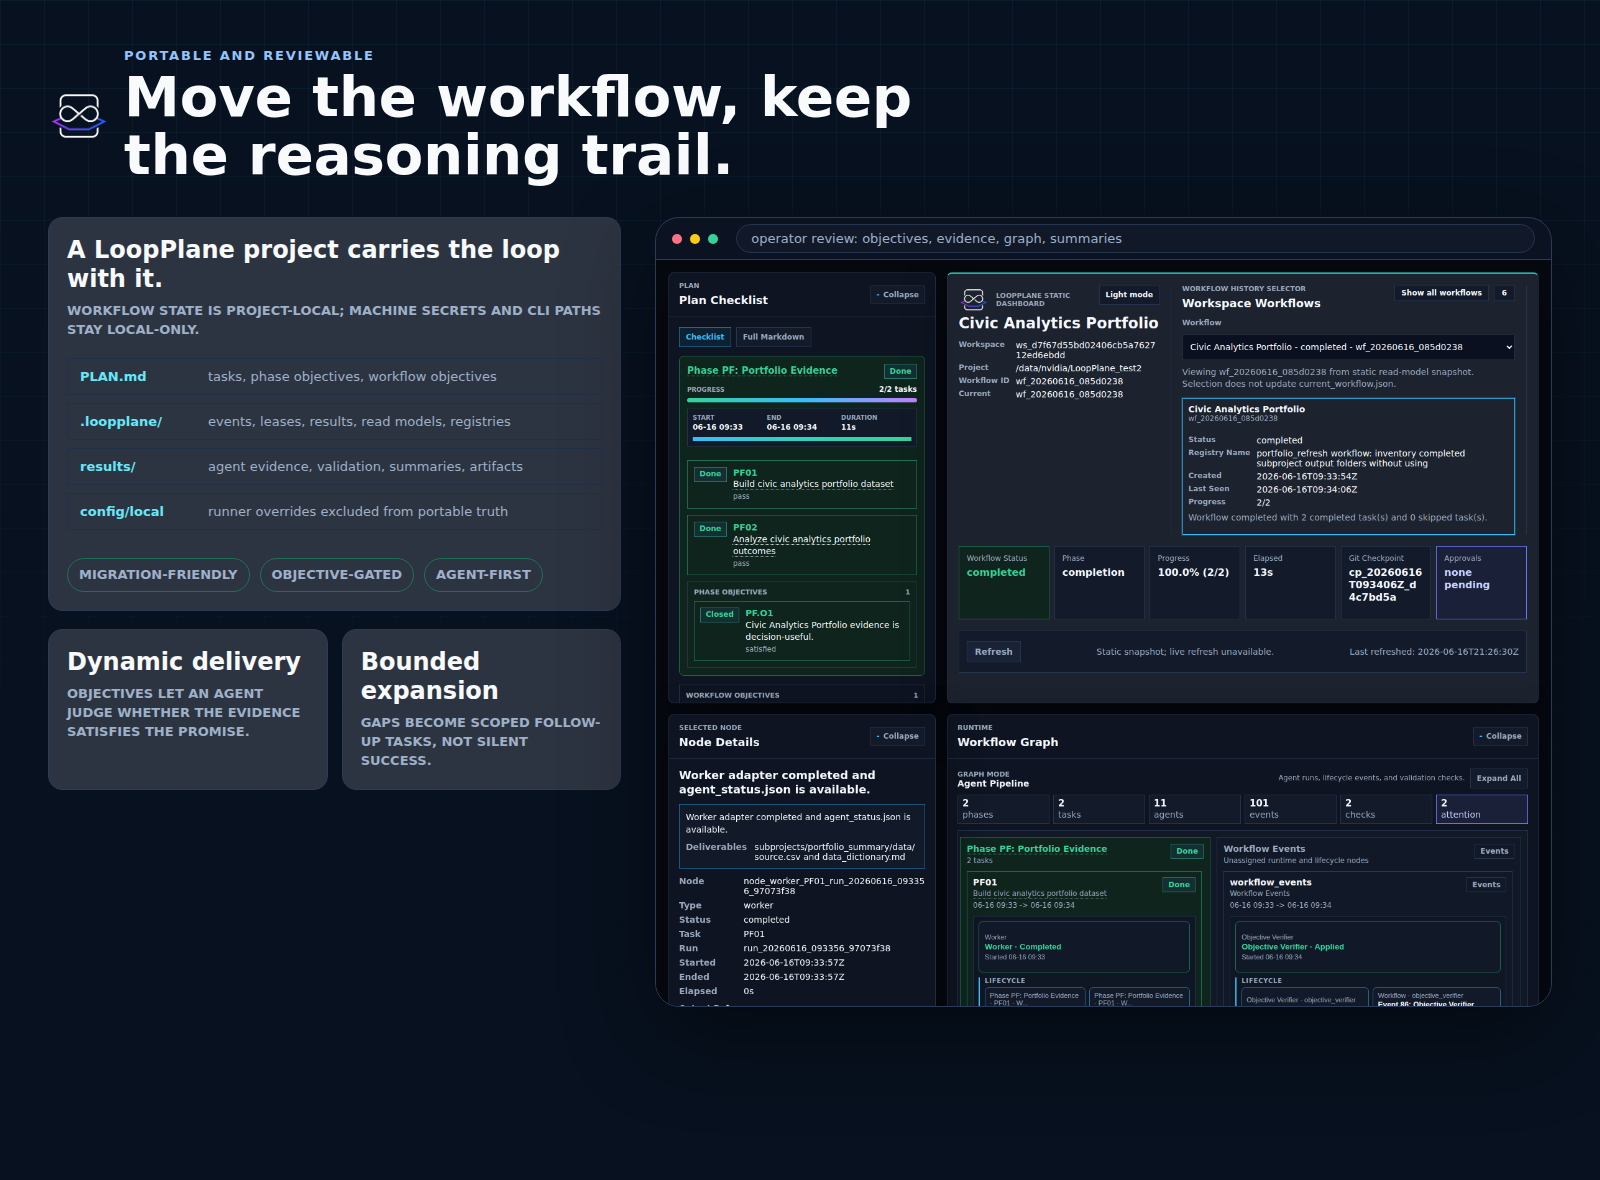
\includegraphics[width=\linewidth]{showcase_surface.png}
\caption{LoopPlane combines a portable workflow package with a dashboard
surface for human review. The dashboard demonstrates usability while remaining
a projection over local workflow records.}
\end{figure}

\begin{figure}[H]
\centering
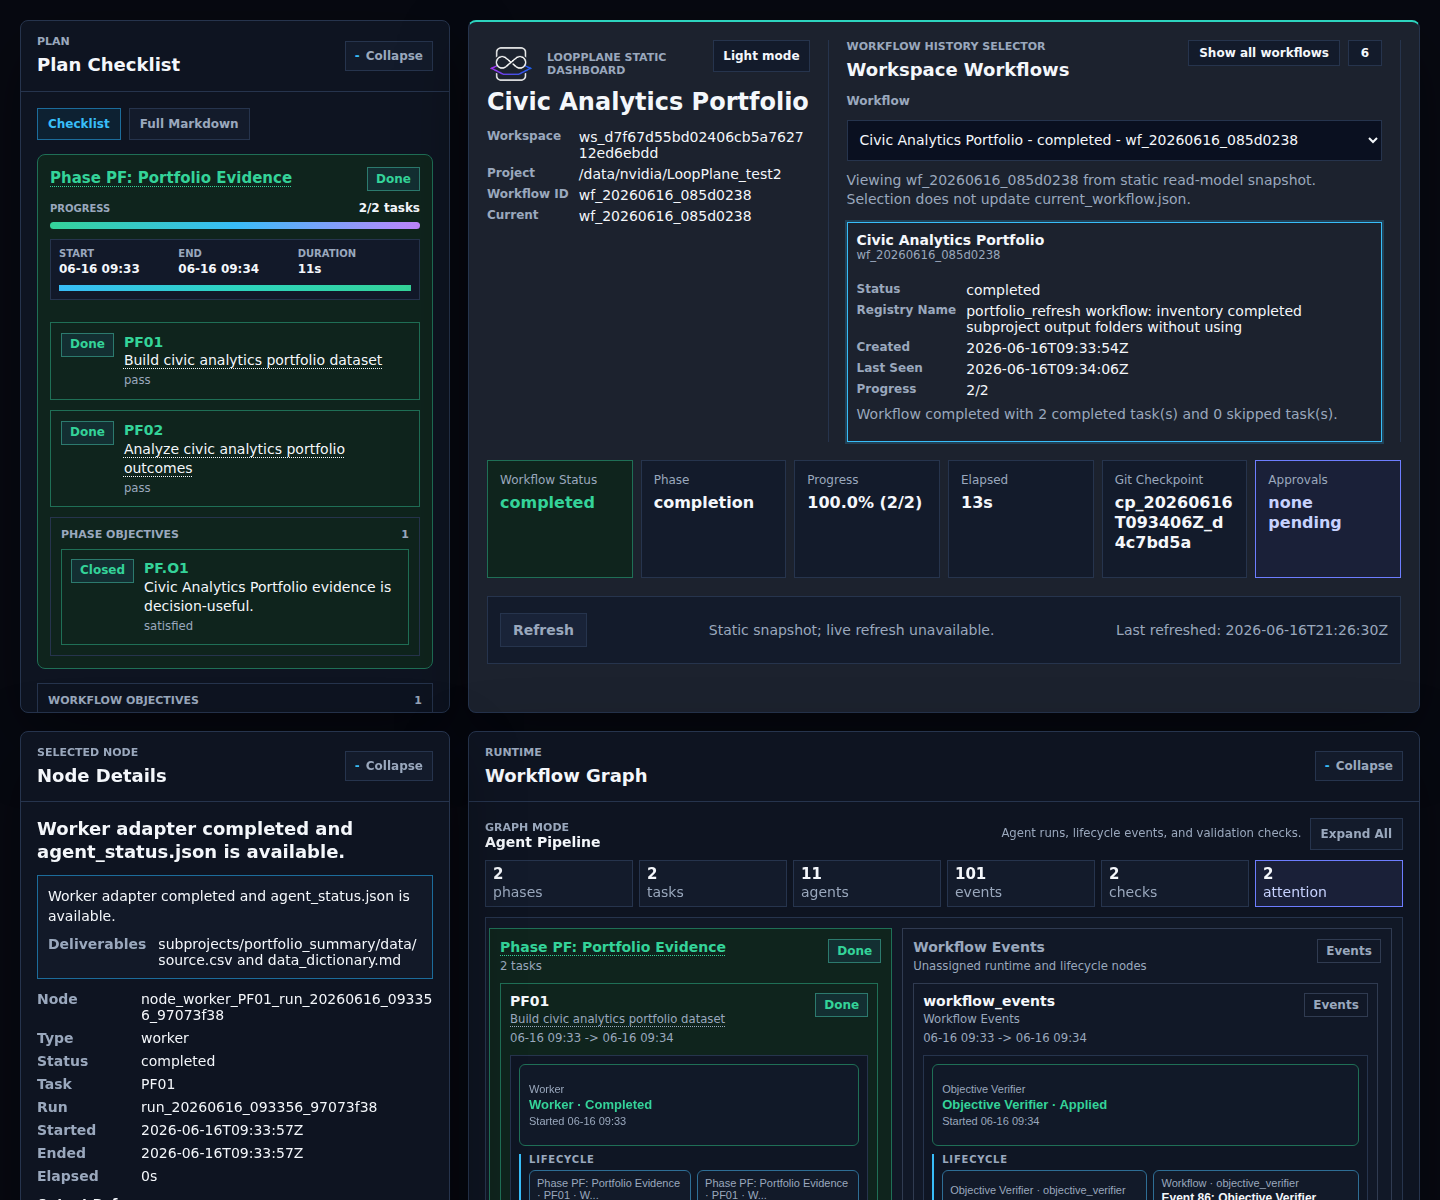
\includegraphics[width=0.9\linewidth]{dashboard_overview.png}
\caption{Operator dashboard showing objective closure, task progress, workflow
history, graph state, selected-node evidence, and control points.}
\end{figure}

\section{Portability and Migration}

The portable workflow model is a product feature. A LoopPlane project carries
its plan, runtime records, results, objective reports, summaries, read models,
and generated review surfaces. Local runner overrides, private paths, and
credentials remain outside portable truth.

This enables practical workflows:

\begin{itemize}
\item archive a completed agent workflow as a durable project artifact;
\item resume an unfinished workflow on another machine;
\item hand a workflow to another reviewer without losing context;
\item compare workflows through generated read models;
\item preserve a clean boundary between local evidence and presentation.
\end{itemize}

\section{Example Workflow Surface}

A representative workflow can complete tasks, close objectives, generate
structured artifacts, and surface evidence through both summaries and dashboard
read models. The important product behavior is not the particular dataset; it
is the preserved chain from plan to evidence to objective closure to reviewable
surface.

\begin{table}[H]
\centering
\begin{tabular}{p{0.34\linewidth}p{0.52\linewidth}}
\toprule
Product Signal & User Value \\
\midrule
Task evidence & Artifacts and logs are attached to the workflow record. \\
Objective closure & High-level delivery is judged after evidence exists. \\
Human summaries & Agents explain what changed, what matters, and what remains risky. \\
Read models & Graphs, metrics, feeds, and status are rebuilt from local records. \\
Dashboard & Users can review the loop without reconstructing it manually. \\
\bottomrule
\end{tabular}
\caption{Product behavior demonstrated by a representative workflow.}
\end{table}

\section{Conclusion}

LoopPlane reframes agent automation as a durable, migratable workflow runtime.
Its contribution is the combination of static task execution, dynamic objective
closure, agent-first semantic judgment, bounded self-expansion, local runtime
truth, and user-friendly projections. The result is an agent workflow product
that can continue autonomously, remain auditable, and travel with its reasoning
trail intact.

\end{document}
